\section{INLA for Gaussian Data}
In this section we will look at the smoothing of a time series and how to use integrated nested Laplace approximations which we from here on will refer to as INLA.

\subsection{Data exploring}
 
\begin{figure}[h]
    \centering
    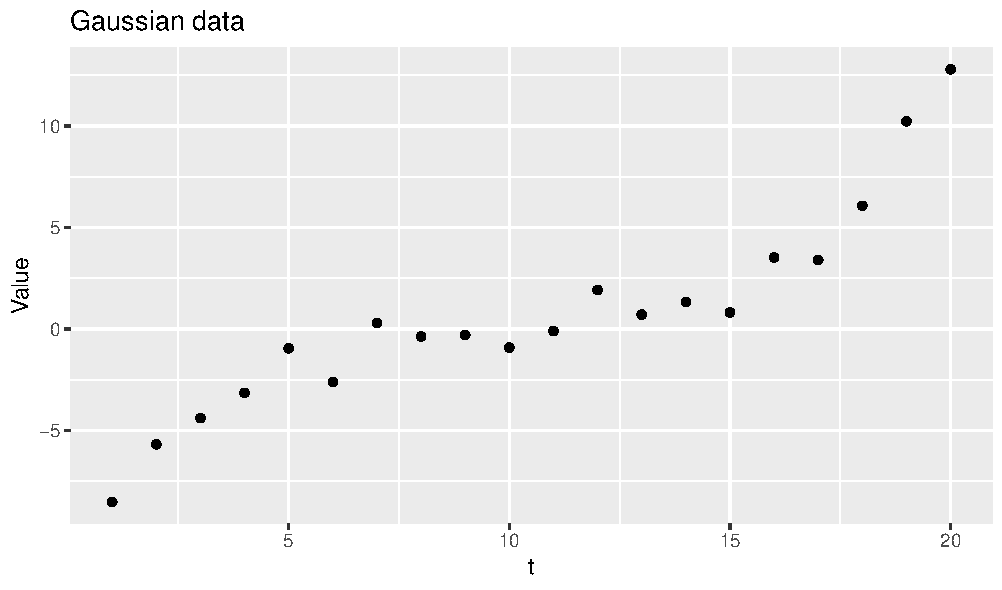
\includegraphics[width=\textwidth]{Images/gaussian_data.pdf}
    \caption{Constructed Gaussian data.}
    \label{fig:gaussian_data}
\end{figure}

In Figure \ref{fig:gaussian_data} vi can see the Gaussian data we want to find the underlying distribution of. We note that it looks like some of the previous values influence the next value in the time series. 


\subsection{Latent Gaussian model}

As given in the problem text, we assume that given the vector $\eta = (\eta_1...\eta_T)$ the observations $y_k$ are independent and Gaussian distributed, having mean $\eta_t$. The known unit variance is $y_t|\eta_t = \mathcal{N}(\eta_t, 1); t = 1,...,T$, and there is a smooth effect of time which the linear predictor is linked to, $\eta_t = f_t$. 

We are choosing a second order Random Walk model as the prior distribution for the vector \textbf{f} $= (f_1,...,f_T)$ model the temporal effects of the covariates. As $\eta_t = f_t$, we have that 

\begin{align} [\label{RW_prior}]
    \pi(\textbf{f}|\theta) = \pi(\textbf{\eta}|\theta) \propto
    \theta^{(T-2/2)} \text{exp} \Bigg{  -\frac{\theta}{2} \sum_{t = 3}^T (f_t - 2f_{t-1} + f_{t-2})^2  \Bigg} = \mathcal{N}(\textbf{0}, \textbf{Q}(\theta)^{-1}).
\end{align}

To find the precision matrix for our model, we expand the expression for $\textbf{Q}(\theta)$ from \ref{RW_prior}. We then have that 

\begin{align}
    \textbf{Q}(\theta) = \sum_{t = 3}^T (f_t - 2f_{t-1} + f_{t-2})^2
\end{align}






- Skriv inn modellene fra oppgaveteksten 

- skriv in hva pressicion matrixen Q blir, det gjør det tydeligere at det er en GMRF siden den er sparse

\todo[color = yellow]{Hvis du fokuserer på å få inn alle plottene og skrive innn likningene så kan jeg vet skrive forståelsestingene på tirsdag. I hvert fall er g6t5fr5det fint om du tar det i den rekkefølgen :D  }

- forklar at det er en Gaussian latent model og GMRF

- It is a latent gausian model, these are a subclass of the structured additive regression models - > y belongs to the exponential family. In addition all latent variabler have gausian priors. 

%Dette er structured additiv model
\begin{equation}
\begin{split}
    g(\mu_i) = \eta_i = \alpha + \sum_{k = 1}^{n_\beta} \beta_k z_{mi} + \sum_{j = 1}^{n_f}f^{(j)}(u_{ji}) + \epsilon_i
\end{split}
\end{equation}

- i tillegg må the latent field være cond indep, i vårt tilfelle være $\eta_i$ ene
- siste punkt er få hyperparametere



%As $f|\theta$ is Gaussian distributed with mean $0$ and precision matrix $\textbf{Q}(\theta)$, we need to define the precision matrix of the model in order to use INLA. The precision matrix is defined as 



\subsection{Gibbs sampling algorithm for $f(\eta, \theta |y)$}

First we implement a Gibbs sampling algorithm for $f(\eta, \theta |y)$. To do so we need the full conditional of both $\pi(\theta|\eta, y)$ and $\pi(\eta|\theta, y)$. They are:

- skriv inn the full conditional for $\pi(\theta|\eta, y)$ og $\pi(\eta|\theta, y)$

\begin{align}
    \pi(\theta| \eta, y) = \pi(y|\eta) \cdot \pi(\eta|\theta) \cdot \pi(\theta) \propto \pi(\eta|\theta) \cdot \pi(\theta) \nonumber \\
    = \theta^{\frac{(T-2)}{2}} \cdot exp \Big( \eta^T Q \frac{\theta}{2} \eta \Big) \cdot exp(\theta) \nonumber \\
    = exp \Big(  \theta \big(1 + \frac{\eta^T Q \eta}{2}  \big) \theta^{\frac{(T-2)}{2}}  \Big), 
\end{align}

and 
\begin{align}
    \pi(\eta | \theta, y) = 
\end{align}

We note that the full conditional for $\theta$ is a gamma distributed with shape parameter $\alpha = T/2$ and scale parameter $\beta = 1/(\frac{1}{2}\cdot (1 + \eta^T Q \eta))$ and the full conditional for $\eta$ is multivariate normal distributed with mean $\boldsymbol{\mu} = \boldsymbol{y}(I + Q \theta)^{-1}$ and variance covariance matrix given by $\Sigma = (I + Q \theta)^{-1}$. $Q$ is teh precision matrix defined in ....
$I$ is the identity matrix and $y$ are the values of the dataset for each time as seen in Figure \ref{fig:gaussian_data}. 


\lstinputlisting[language=R, firstline=56, lastline=67]{Code/INLA.R}

Now we are ready to implement the Gibbs sampling for $f(\eta, \theta | \boldsymbol{y})$. Firstly, we propose a new value for $\theta$ using the full conditional $\pi(\theta|\eta, \boldsymbol{y})$ then we propose a new value for $\eta$ using the full conditional $\pi(\eta|\theta, \boldsymbol{y})$. 

\lstinputlisting[language=R, firstline=69, lastline=86]{Code/INLA.R}

We run with initial values for $\theta = 0$ and $\eta$ a random sample from the ful lconditional of $\eta$ given the initial condition for $\theta$.

\lstinputlisting[language=R, firstline=88, lastline=100]{Code/INLA.R}

Since this is a MCMC algorithm we nee dto evaluate the burn in period. 


\subsubsection{Estimate for the posterior marginal for the hyperparameter $\pi(\theta|y)$}
\begin{figure}[h!]
    \centering
    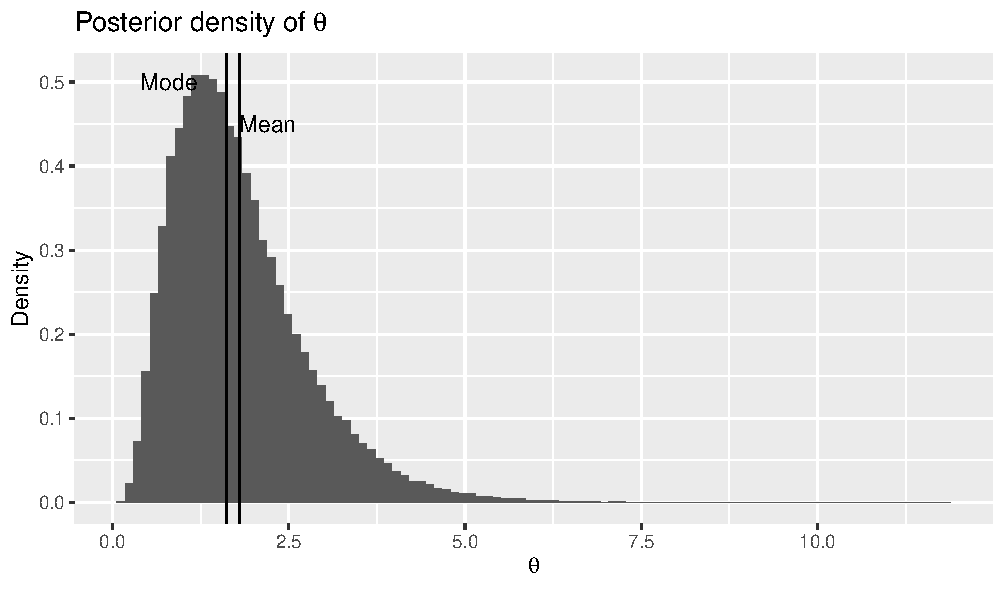
\includegraphics[width=\textwidth]{Images/post_theta_mcmc.pdf}
    \caption{Plot of the estimate for the posterior marginal for the hyperparameter $\pi(\theta|y)$.}
    \label{fig:post_theta_mcmc}
\end{figure}

\subsubsection{Estimate of the smooth effect using the mean and pointwise a $95 \%$ confidence bound around the mean}
\begin{figure}[h]
    \centering
    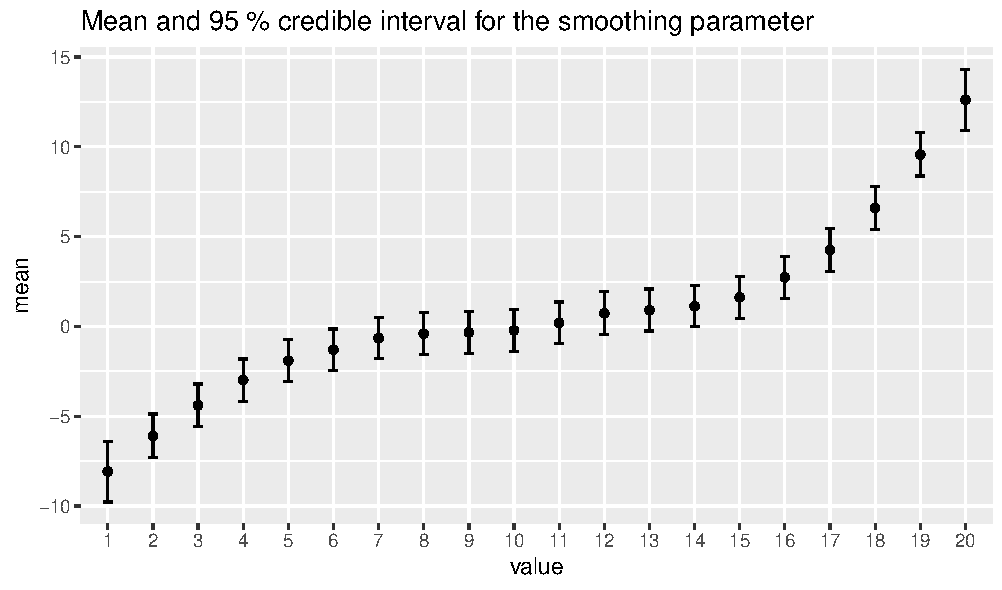
\includegraphics[width=\textwidth]{Images/post_eta_mcmc.pdf}
    \caption{Plot of the mean and the $95\%$ credible interval for the smoothing parameter $\eta$. }
    \label{fig:post_eta_mcmc}
\end{figure}

\subsection{Approximating the posterior marginal for the hyperparameter $\theta$, $\pi(\theta|y)$ using the INLA scheme}

\begin{figure}[h!]
    \centering
    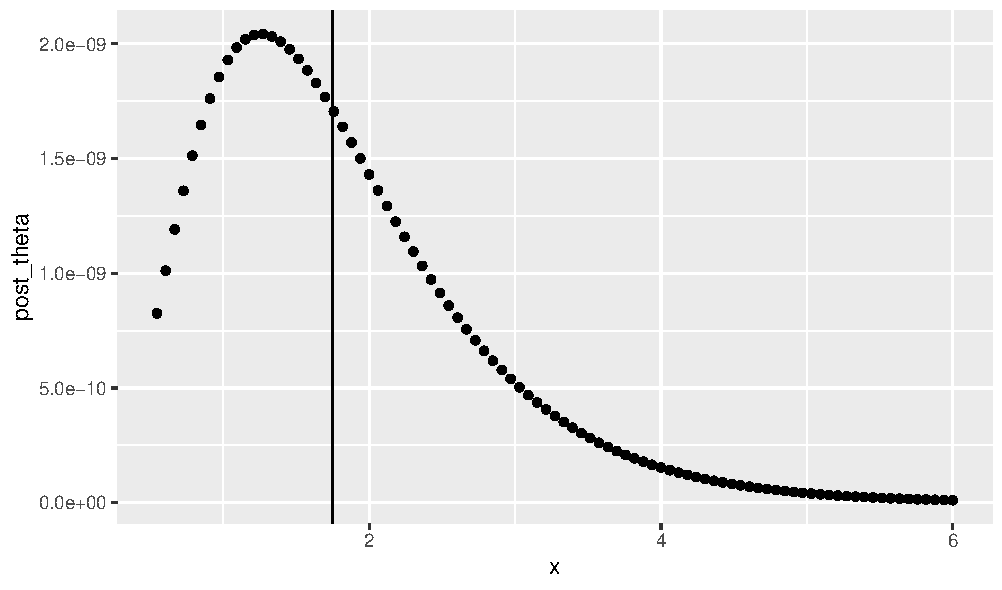
\includegraphics[width=\textwidth]{Images/post_theta_inla.pdf}
    \caption{Plot of the estimate for the posterior marginal for the hyperparameter $\pi(\theta|y)$ using the INLA scheme.}
    \label{fig:post_theta_inla}
\end{figure}
 
 
\subsubsection{Approximation for $\pi(\theta|y)$}


- veldig mye av disse tingene står som kladd i de pdf ene jeg sendte deg så se gjerne der for inspirasjon-


\subsection{Implementing the approximation of the marginal posterior for the smooth effect, $\pi(\eta_i | y)$}

\begin{figure}[h!]
    \centering
    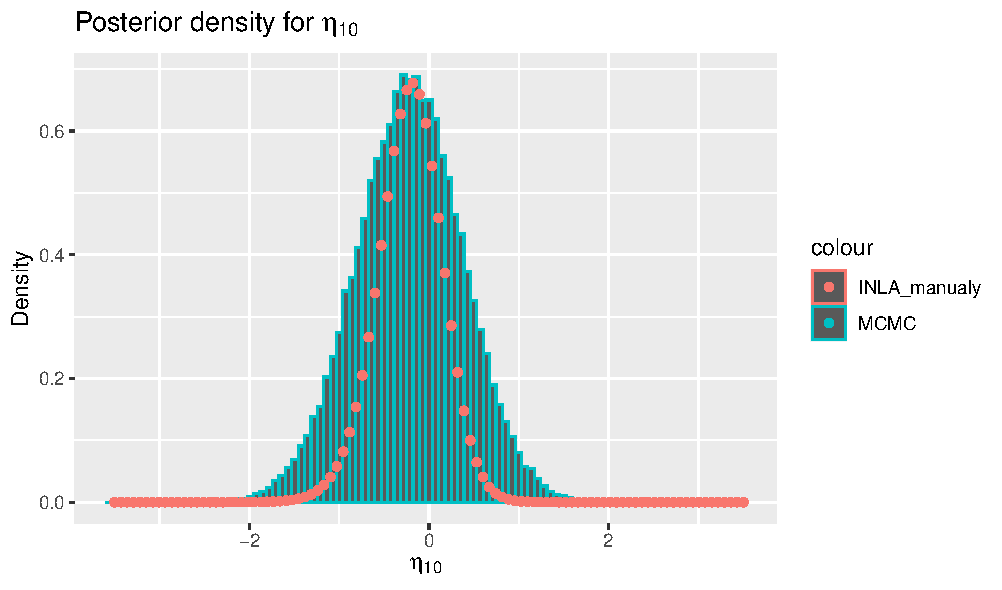
\includegraphics[width=\textwidth]{Images/post_eta_inla.pdf}
    \caption{Plot of the estimate for the posterior marginal for the smoothing effect $\pi(\eta_i|y)$ using the INLA scheme.}
    \label{fig:post_eta_inla}
\end{figure}



\subsection{Using the inla() - function in R to implement the model,and comparing the results}


\begin{figure}[h]
    \centering
    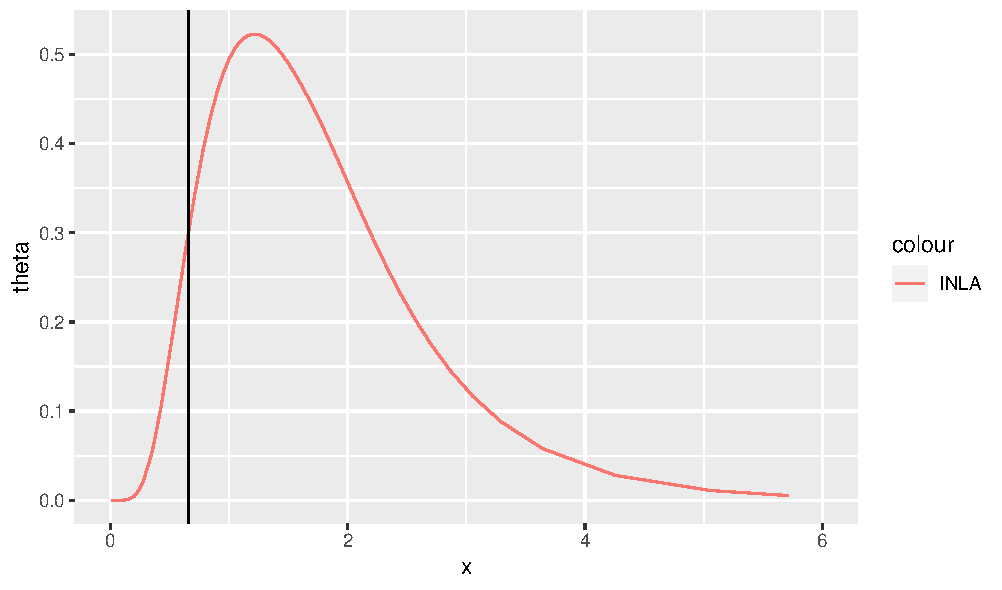
\includegraphics{Images/R_inla_theta.pdf}
    \caption{Plot of the estimates $\theta$ using the inla()-function in the R-inla library}
    \label{fig:r_inla_theta}
\end{figure}

\begin{figure}[h]
    \centering
    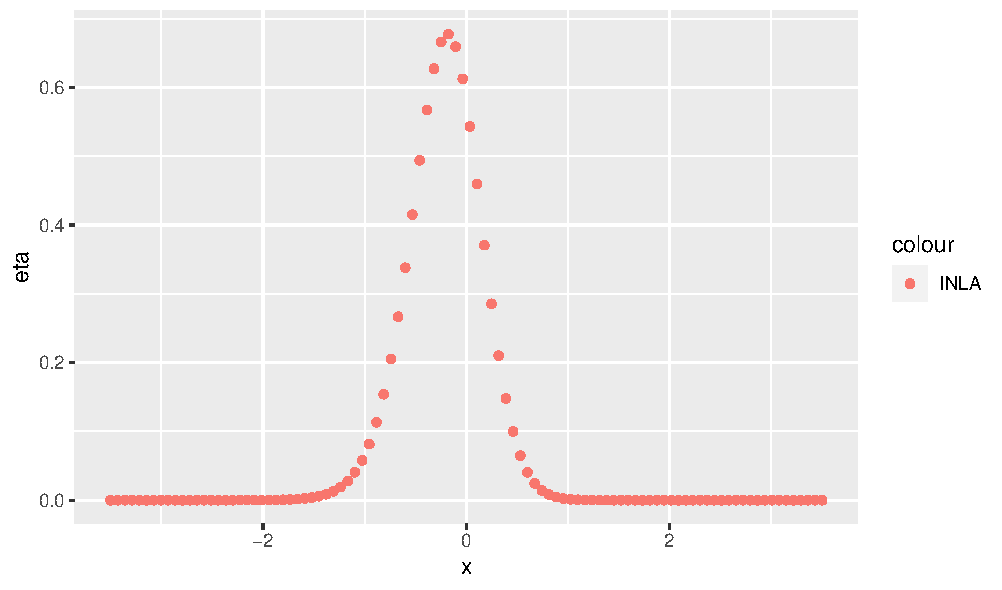
\includegraphics{Images/R_inla_eta.pdf}
    \caption{Plot of the estimates of the smoothing parameter $\eta$ using the inla()-function on the R-inla library.}
    \label{fig:r_inla_eta}
\end{figure}

\begin{figure}[h]
    \centering
    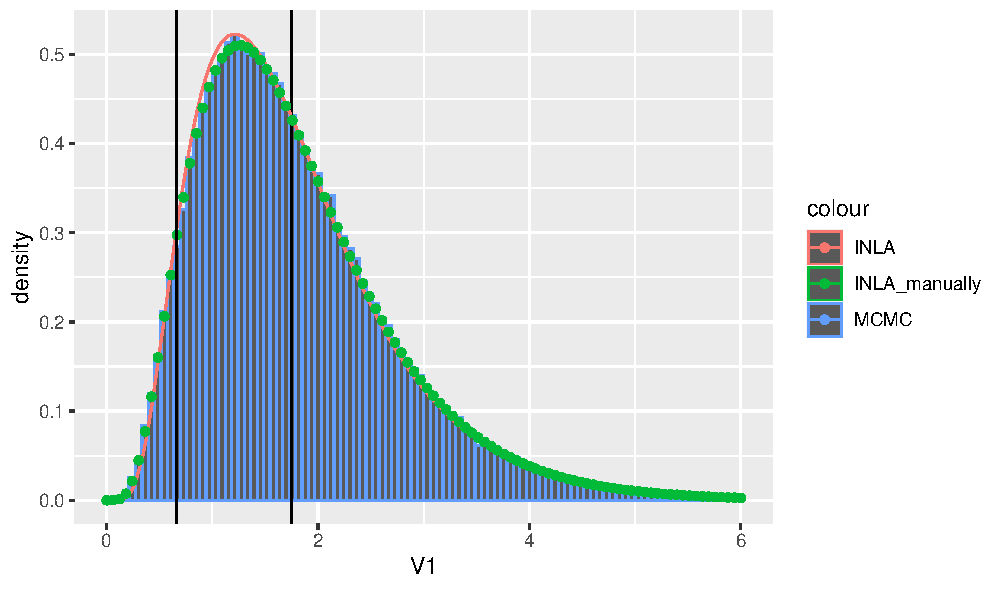
\includegraphics{Images/theta_comparison.pdf}
    \caption{Plot of estimated hyperparameter $\theta$ for MCMC, manually implemented INLA and INLA implemented using R-inla().}
    \label{fig:theta_comparison}
\end{figure}

\begin{figure}[h]
    \centering
    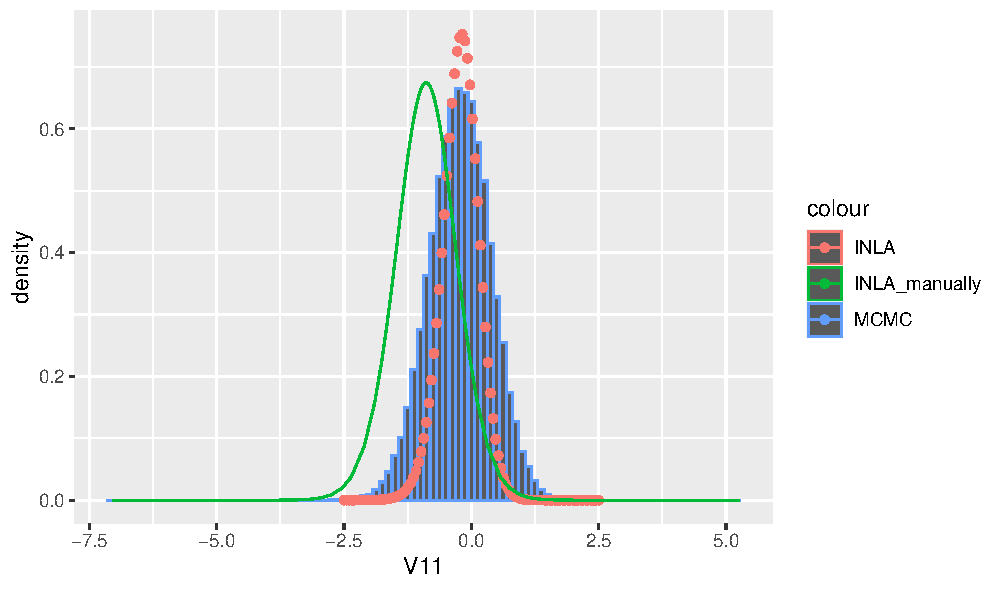
\includegraphics{Images/smoothing_comparison.pdf}
    \caption{Plot of estimated smoothing parameter $\eta$ for MCMC, manually implemented INLA and INLA implemented using R-inla().}
    \label{fig:smoothing_comparison}
\end{figure}
